\section{Evaluation}\label{sec:evaluation}

\begin{figure*}
    \centering
    \begin{subfigure}{0.49\textwidth}
        \centering
        \includegraphics[width=\textwidth]{diagrams/injection/original.jpg}
        \caption{Original image with some fires.\newline}
        \label{fig:injection-orig}
    \end{subfigure}
    \begin{subfigure}{0.49\textwidth}
        \centering
        \includegraphics[width=\textwidth]{diagrams/injection/random_combined_diagonal.jpg}
        \caption{Fires randomly injected uniformly across the map. Composite of 3 images, with intensity of the fires increasing from top to bottom.}
        \label{fig:injection-random}
    \end{subfigure}
    \caption{An overview of the possible ways an attacker can manipulate the output of the forest fire detection algorithm by overshadowing the downlinked data. In each image, forest fires detected by the algorithm are highlighted in yellow, orange, and red in increasing order of intensity.}
    \label{fig:injection}
\end{figure*}

\begin{figure}
    \includegraphics[width=\columnwidth]{diagrams/injection/masked_0.jpg}
    \caption{MODIS image with legitimate fires masked out.}
    \label{fig:injection-masked}
\end{figure}

In order to attack systems which rely upon Earth observing satellite data, the attacker must synthesise a malicious signal which decodes to the desired raw data.
When processed, this raw data will either poison the targeted satellite-derived dataset, or exploit a stage in the processing pipeline itself.
Then the attacker must overshadow a genuine broadcast with sufficient amplitude such that the targeted receiver decodes the attacker's signal.

In this section, we demonstrate the feasibility of each of these objectives with respect to a case study on FIRMS, NASA's forest fire detection system.
We firstly show in Section~\ref{sec:effects-on-processing-systems} how an attacker can generate an attack sequence which results in the injection of ficticious forest fires, the masking of existing ones, or the exploitation of vulnerabilities in the protocol decoding stages.
Since existing implementations of the EOS protocols are intended for decoding only, we firstly implement libraries to reencode the data.
We build upon these to demonstrate our attacks end-to-end on the FIRMS software, resulting in color-corrected images overlaid with the detected forest fires.

We go on to demonstrate the feasibility of the attack using only commercially available equipment through a series of radio overshadowing simulations.
The results demonstrate that a ground-based attacker can achieve the required overshadowing of a highly directional dish, for the budget of a motivated hobbyist.

\subsection{Effects on downlink processing systems}\label{sec:effects-on-processing-systems}

\subsubsection{Case Study: Injecting ficticious forest fires}

% If more time: describe the engineering re packet splitting across boundaries etc.

To successfully inject forest fires, an attacker needs to manipulate the infrared channels of MODIS packets within the downlinked data.
This data can either be obtained from distributed digital archive centers~\cite{ladsweb} beforehand, or in real time with access to a satellite dish.
In this example, the attacker is injecting forest firest at specific geographic coordinates, and so obtains data representing the desired target beforehand.
However, since all the information required to generate the data is present either from the known orbital parameters or within the data stream itself, forest fires could be similarly injected in real time.

% If more time: explain how the correct data is found wrt certain coordinates, in the long list
Data is available for download in the \textit{Level 0} format, which consists of MODIS SPP packets already decoded from the CADUs.
The archive lists packet data broken into short sequences according to the time at which the data was captured.
The attacker selects a sequence of packets corresponding to their targeted area, using the predictable orbital characteristics of the satellite to calculate the overpass time.

Once received, the attacker needs to modify the infrared sensor channels to draw fires at the desired locations.
By running the packet sequence through \textit{MODISL1DB\_SPA}, the attacker obtains the precise geographical coordinates of the boundaries of the image.
The attacker can target specific pixels in the image, since the sequence of packets encodes a scan over the image in a predicable pattern.
Specifically, the image is laid out as horizontal scan lines across the frame.
The number of the scan line is indicated in the secondary header, with the \textit{frame data count} increasing linearly throughout the scan.

Using this method, the attacker can determine the precise packets which, when modified will lead to the addition of forest fires at the desired coordiates.
However, since MOD14\_SPA detects fires through local peaks~\cite{mod14Manual}, the attacker can't write uniform values across large sequences of packets.
Forest fires are detected if instead the values within the desired area are set according to a random distribution.

Additionally, in order to have the image decode correctly, the attacker must be careful not to modify any non-sensor packets within the sequence.
For example, engineering packets are interspersed regularly throughout the sequence, which contain crucial timing information later used in the alignment of the scan lines between sensors.
Engineering packets are distinguished uniquely with a frame data count of zero, so an exception must be made to leave such packets unmodified.
Figure ~\ref{fig:interleave} demonstrates the partial result of an image with this timing data overwritten.

Finally, the attacker must reencode the SPP packet sequence into the CADU structure, aligning the packets within the structure accordind to the specification, recalculating the checksums, and applying the Viterbi encoding.
Figures~\ref{fig:injection} and~\ref{fig:location-injection} show the results of the FIRMS software stack within IPOPP decoding the resulting signal.


%Show the pipeline which results in the injection of ficticious fires, and the results
%Get a bit of info from Josh about how his pixel alignment works

\subsubsection{Case Study: Masking existing forest fires}

The attacker can also seek to mislead the fire detection algorithm through masking existing forest fires.
Unlike the case of creating ficticious fires, the attacker doesn't need to perform geolocation of the image, greatly simplifying the operation of processing the packets.
As a result, it becomes significantly easier to perform the attack in real time.

Data in this case study is instead obtained directly from an attacker receiver.
The bit sequence from the decoder must firstly be byte aligned and divided into CADUs, derandomised through Viterbi decoding depending on the satellite mode, and then error corrected according to the CADU checksum.
The result is an SPP MODIS packet sequence of equivalent form to those obtainable from the online archives.

The attacker can process the packet sequence with low latency, since the operation to each sensor packet is identical.
Specifically, the attacker needs to all of the infrared channels to a roughly uniform value.
Therefore, MOD14\_SPA fails to detect the requisite peaks, and the resulting dataset contains no marked fires.
The results can be seen in Figure~\ref{fig:injection-masked}.

% Show the pipeline for masking forest fires, including a code sample from the part that masks

\subsubsection{Case Study: Exploiting MODIS packet decoding}

\begin{figure}
    \includegraphics[width=\columnwidth]{diagrams/interleave.png}
    \caption{Failure correctly distinguish engineering from sensor data leads to malformed output.}
    \label{fig:interleave}
\end{figure}

Attackers can also seek to disrupt the generation of satellite-derived datasets by exploiting the software which decodes the packets themselves.

In the simplest case, the attacker can take advantage of the noise-resilient properties of the physical layer encoding scheme to deny service.
The data is encoded using \textit{Quadrature phase-shift keying} (QPSK), which encodes only two bits per symbol; as the number of bits encoded per symbol increases, the less resilient the encoding scheme is to noise since decoding relies on detecting increasingly subtle shifts in the carrier wave.
Since each frame begins with a synchronisation header, which the downlink processing systems are designed to preferentially select, the attacker can selectively jam through overshadowing with the header.
This technique has been shown to be effective in other similar scenarios, targeting the collision avoidance system of 802.11 networks~\cite{gummadi2007understanding}.


However, as explored in Section~\ref{sec:attack}, more suble attacks are possible which exploit the decoders for data link layer headers.
Unline the sensor data within, which consists of a densely packed array of 12 bit words, the protocol headers present more possibilities for modification and thus a greater attack surface.

the IPOPP distribution consists of many complex execution pathways, which pass data between multiple applications unsafely.
As a result, it is possible for attacker to embed carefully crafted packets within the injected data, which exploit vulnerabilities when reprocessed.

We take as a case study MODISL1DB\_SPA, the software responsible for unpacking SPP MODIS packets into the intermediate HDF form.
MODISL1DB\_SPA consists of many complex execution pathways, which pass data between multiple applications unsafely.
As a result, it is possible for attacker to embed carefully crafted packets within the injected data, which exploit vulnerabilities when reprocessed.

In decoding the packets, MODISL1DB\_SPA must extract the data and correct corrupted data in the case of failure.
These tasks are performed by the \textit{OceanColor Science Software} (OCSSW)~\cite{ocssw} tools, developed by the OceanColor Data team.
The OCSSW tools are written in C and Fortran, and were originally designed to be run as command line scripts.
They expect a parameter file which describes the location of the data to be processed and supplies options for processing it.

In order to automate processing and correcting the data, Python programs were written which construct the command line arguments and parameter files required for the OCSSW tools, and then invoke a shell to execute them.
These are designed to be higher-level tools for use in analysing and processing the data files on the command line, without requiring knowledge of the complex parameter files.
However, these tools now additionally form the basis of MODISL1DB\_SPA.

In many cases, due to the architecture of the software, the only thing prevent arbitrary code execution are minor configuration issues.
However, in other cases, code execution pathways are possible.
Figure~\ref{fig:code-execution} demonstrates a code excerpt, in which a function sets the output file path name based on the members of a tar file.
Afterwards, this file path is passed untokenized to the shell.
As a result, by passing a malicious tarball in the form of an SPP packet, the attacker can also gain code execution on the user's machine.

\begin{figure*}
    \centering
    \begin{lstlisting}[language=Python]
    def _extract_viirs_sdr(self, tar_path):
        self.file_path = None
        try:
            # orig_path = os.getcwd()
            tar_file = tarfile.TarFile(tar_path)
            tar_members = tar_file.getnames()
            for mbr in tar_members:
                if mbr.startswith('SVM01'):
                    mbr_info = tar_file.getmember(mbr)
                    tar_file.extractall(members=[mbr_info], path='/tmp')
                    self.file_path = os.path.join('/tmp', mbr)
                    break
            tar_file.close()
        except:
            exc_info = sys.exc_info()
            for item in exc_info:
                print(str(item))
    ...

    l0cnst_results = None
    cmd = ' '.join(['l0cnst_write_modis', '-n', self.file_path])
    try:
        l0_out = subprocess.Popen(cmd, shell=True, stdout=subprocess.PIPE,
                                  stderr=subprocess.PIPE).communicate()[0]
    \end{lstlisting}
    \caption{Excerpt of a potentially vulnerable code exectution pathway in the decoding software. The function sets \texttt{self.file\_path} based on parameters parsed from the file at \texttt{tar\_path}. \texttt{self.file\_path} is then passed untokenized to the shell.}
    \label{fig:code-execution}
\end{figure*}

\subsection{Physical-Layer Validation}\label{sec:physical-layer-validation}

In order to demonstrate the feasibility of signal injection attacks on EOS downlink systems in a real-world setting, we perform a simulated analysis of the proposed attacks.
We use ``GNU Radio'' to construct a pipeline which simulates a legitimate downlink signal broadcast from the Terra satellite and demodulated using (QPSK), the physical layer encoding scheme used in the EOS radio stack.
We also simulate an attacker-injected signal added to the legitimate signal and demodulated by the same process.
By varying the gain on the injected signal and measuring the Bit Error Rate (BER) of the decoded bytes, we can assess the transmission power required for the attack to succeed.
The concept of this signal overshadowing attack is introduced in Figure~\ref{fig:attack-illustration}, and an overview of the experimental configuration is shown in Figure~\ref{fig:overshadowing_pipeline}.
% The source code is also available alongside our other artifacts (\textbf{TODO}).

In order to carry out these simulations with a reasonable degree of confidence that they accurately represent the real world, we establish simulation parameters based on known characteristics of the EOS radio systems.
We use the link budget established in~\cite{quinnNew2003} to establish the Effective Isotropic Radiated Power (EIRP) and free-space path loss of the radio signals transmitted by the Aqua and Terra satellites, as well as the antenna gain for signals within the beam of the receiver, and losses within the signal processing pipeline.
We also look at the specification for a commercial EOS ground station to understand how the hardware compares to NASA's ground stations~\cite{dartcomsystemsltdXBand2021}.
On the attacker's side, we use the following standard formula for computing Free-Space Path Loss (FSPL):
\begin{align}
    \text{FSPL}_{\text{dB}} = 20\log_{10}(d) + 20\log_{10}(f) - 147.55, \label{eq:fspl}
\end{align}
where $d$ is the distance from the receiver in meters, and $f$ is the frequency in hertz.
We use the reference antenna radiation pattern given by the International Telecommunication Union in~\cite{itu2022antenna} to estimate the out-of-beam gain of the receiver to be approximately $-10.0$\,dB.
These key values are summarized in Table~\ref{tab:experimental-values}.

We take a range of values for the signal strength at the receiver, between $-100$ and $0$\,dBm.
Received signal strength can be expressed as a function of the attacker's EIRP and distance from the receiver, enabling us to observe the bit error rate as we vary either of these parameters.
We do not accurately model system losses -- since these are consistent between the victim and attacker, we assume their effect on the outcome of the experiment is negligible.
This is verified to be the case by performing the same experiment across a range of noise values and confirming that the result changes by a negligible amount, as seen in Figure~\ref{fig:overshadowing_ber}.
For the main experiments, we set the background noise voltage to $1\,$\textmu V and the system noise to $200$\,mV, resulting in a bit error rate below the $5$\% required for the system to function.

\begin{figure}
    \centering
    \includegraphics[width=\columnwidth]{diagrams/overshadowing_pipeline.pdf}
    \caption{An overview of the GNU Radio pipeline used to provide experimental validation for the overshadowing attacks. IQ samples are indicated in blue, bitstreams in magenta.}
    \label{fig:overshadowing_pipeline}
\end{figure}

\begin{table}
    \resizebox{\columnwidth}{!}{%
    \begin{tabular}{lcc}
        \toprule
        & Victim & Attacker \\
        \midrule
        EIRP (dBm) & $44.4$ & $[0 \dots 100]$ \\
        Distance $d$ (km) & $\sim 713$ & $[0 \dots 10]$ \\
        Free-Space Path Loss (dB) & $179.0$ & $\text{FSPL}_{\text{dB}}(d)$ \\
        Amplitude Multiplier $\left(m = 10^{\frac{\text{EIRP}_{\text{dB}}-\text{FSPL}_{\text{dB}}}{20}}\right)$ & $1.86 \cdot 10^{-7}$ & $m$  \\
        Antenna Gain $g_A$ (dB) & $44.1$ & $-10.0$ \\
        Antenna Amplitude Multiplier $\left( m_A = 10^{\frac{g_A}{20}} \right)$ & $160$ & $0.316$ \\
        System Losses (dB) & $3.7$ & $3.7$ \\
        \bottomrule
    \end{tabular}%
    }
    \caption{Key values used in overshadowing simulations.}
    \label{tab:experimental-values}
\end{table}

\begin{figure}
    \centering
    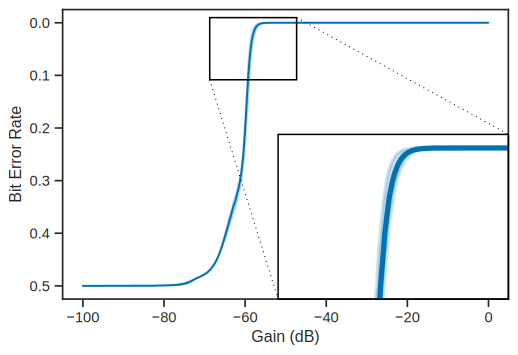
\includegraphics[width=\columnwidth]{diagrams/overshadowing_ber_2.pdf}
    \caption{Error rate of attacker-injected bits as the signal strength at the receiver increases. The small shaded region represents the range of values under different levels of background and system noise.}
    \label{fig:overshadowing_ber}
\end{figure}

The immediate results of our experiment are shown in Figure~\ref{fig:overshadowing_ber}, which compares the signal strength at the receiver to the BER of the injected signal.
In order to understand these results in a meaningful sense, we need to instead consider the factors directly controlled by the attacker: the EIRP of the transmitted signal, and the distance between the attacker and the receiver.
We take the EIRP and subtract FSPL (computed from distance using Equation~\ref{eq:fspl}) to get the received signal strength.

We see the results in Figure~\ref{fig:distance_eirp}, displaying the BER of the injected signal across a range of EIRPs and distances.
This allows us to better understand the threat model initially established in Section~\ref{sec:threat-model}.
The datasheets for the COTS radio equipment described in this section has an EIRP of up to $49$\,dBm -- we therefore know from our experimental results that an attacker with access to this equipment can carry out overshadowing attacks from a distsance of up to $0.71$\,km~\cite{endurosat:xbandtransmitter,endurosat:xbandantenna}.
With access to a more powerful amplifier, the feasible attack range can be extended significantly; an organized criminal group or nation-state level attacker could reasonably be assumed to have access to these.

We conclude from these results that there is cause for concern regarding overshadowing attacks on NASA ground stations -- a motivated hobbyist with a budget of approximately $30,000$ EUR can carry out attacks from almost 1\,km away, and attackers with greater means can do so from an even greater distance.
Furthermore, it is difficult to prevent overshadowing attacks without some method of validating the authenticity of the received signal, and locating the attacker requires a specialized setup to triangulate the signal's origin.
This has implications beyond the attacks described in this paper, demonstrating that all downlink processing systems should be regarded as untrusted unless the data link is authenticated in some way.